\section{Results}

\subsection{\emph{FOXA1} is essential for prostate cancer proliferation}

We interrogated FOXA1 expression levels across cancer types.
We find that FOXA1 mRNA is consistently the most abundant in prostate tumours compared to 25 other cancer types across patients (\Cref{fig:FOXA1_fig1}a), ranking in the 95th percentile for 492 of 497 prostate tumours profiled in TCGA (\Cref{fig:FOXA1_figs1}a).
Using the same dataset we also find that FOXA1 is the most highly expressed out of 41 other Forkhead Box (FOX) factors in prostate tumours (\Cref{fig:FOXA1_figs1}b).
We next analyzed expression data from DEPMAP and observed FOXA1 to be most highly expressed in prostate cancer cell lines compared to cell lines of other cancer types (\Cref{fig:FOXA1_figs2}a).
Amongst the eight prostate cancer cell lines in the dataset (22Rv1, DU145, LNCaP, MDA-PCa-2B, NCI-H660, PrECLH, PC3, and VCaP), FOXA1 mRNA abundance is above the 90th percentile in all but one cell line (PrECLH) compared to the \> 56,000 protein coding and non-protein coding genes profiled (\Cref{fig:FOXA1_figs2}b).
These new results gained from the TCGA and DEPMAP validate previous understanding that FOXA1 is one of the highest expressed genes in prostate cancer \cite{tsourlakisFOXA1ExpressionStrong2017}.

\begin{figure}
  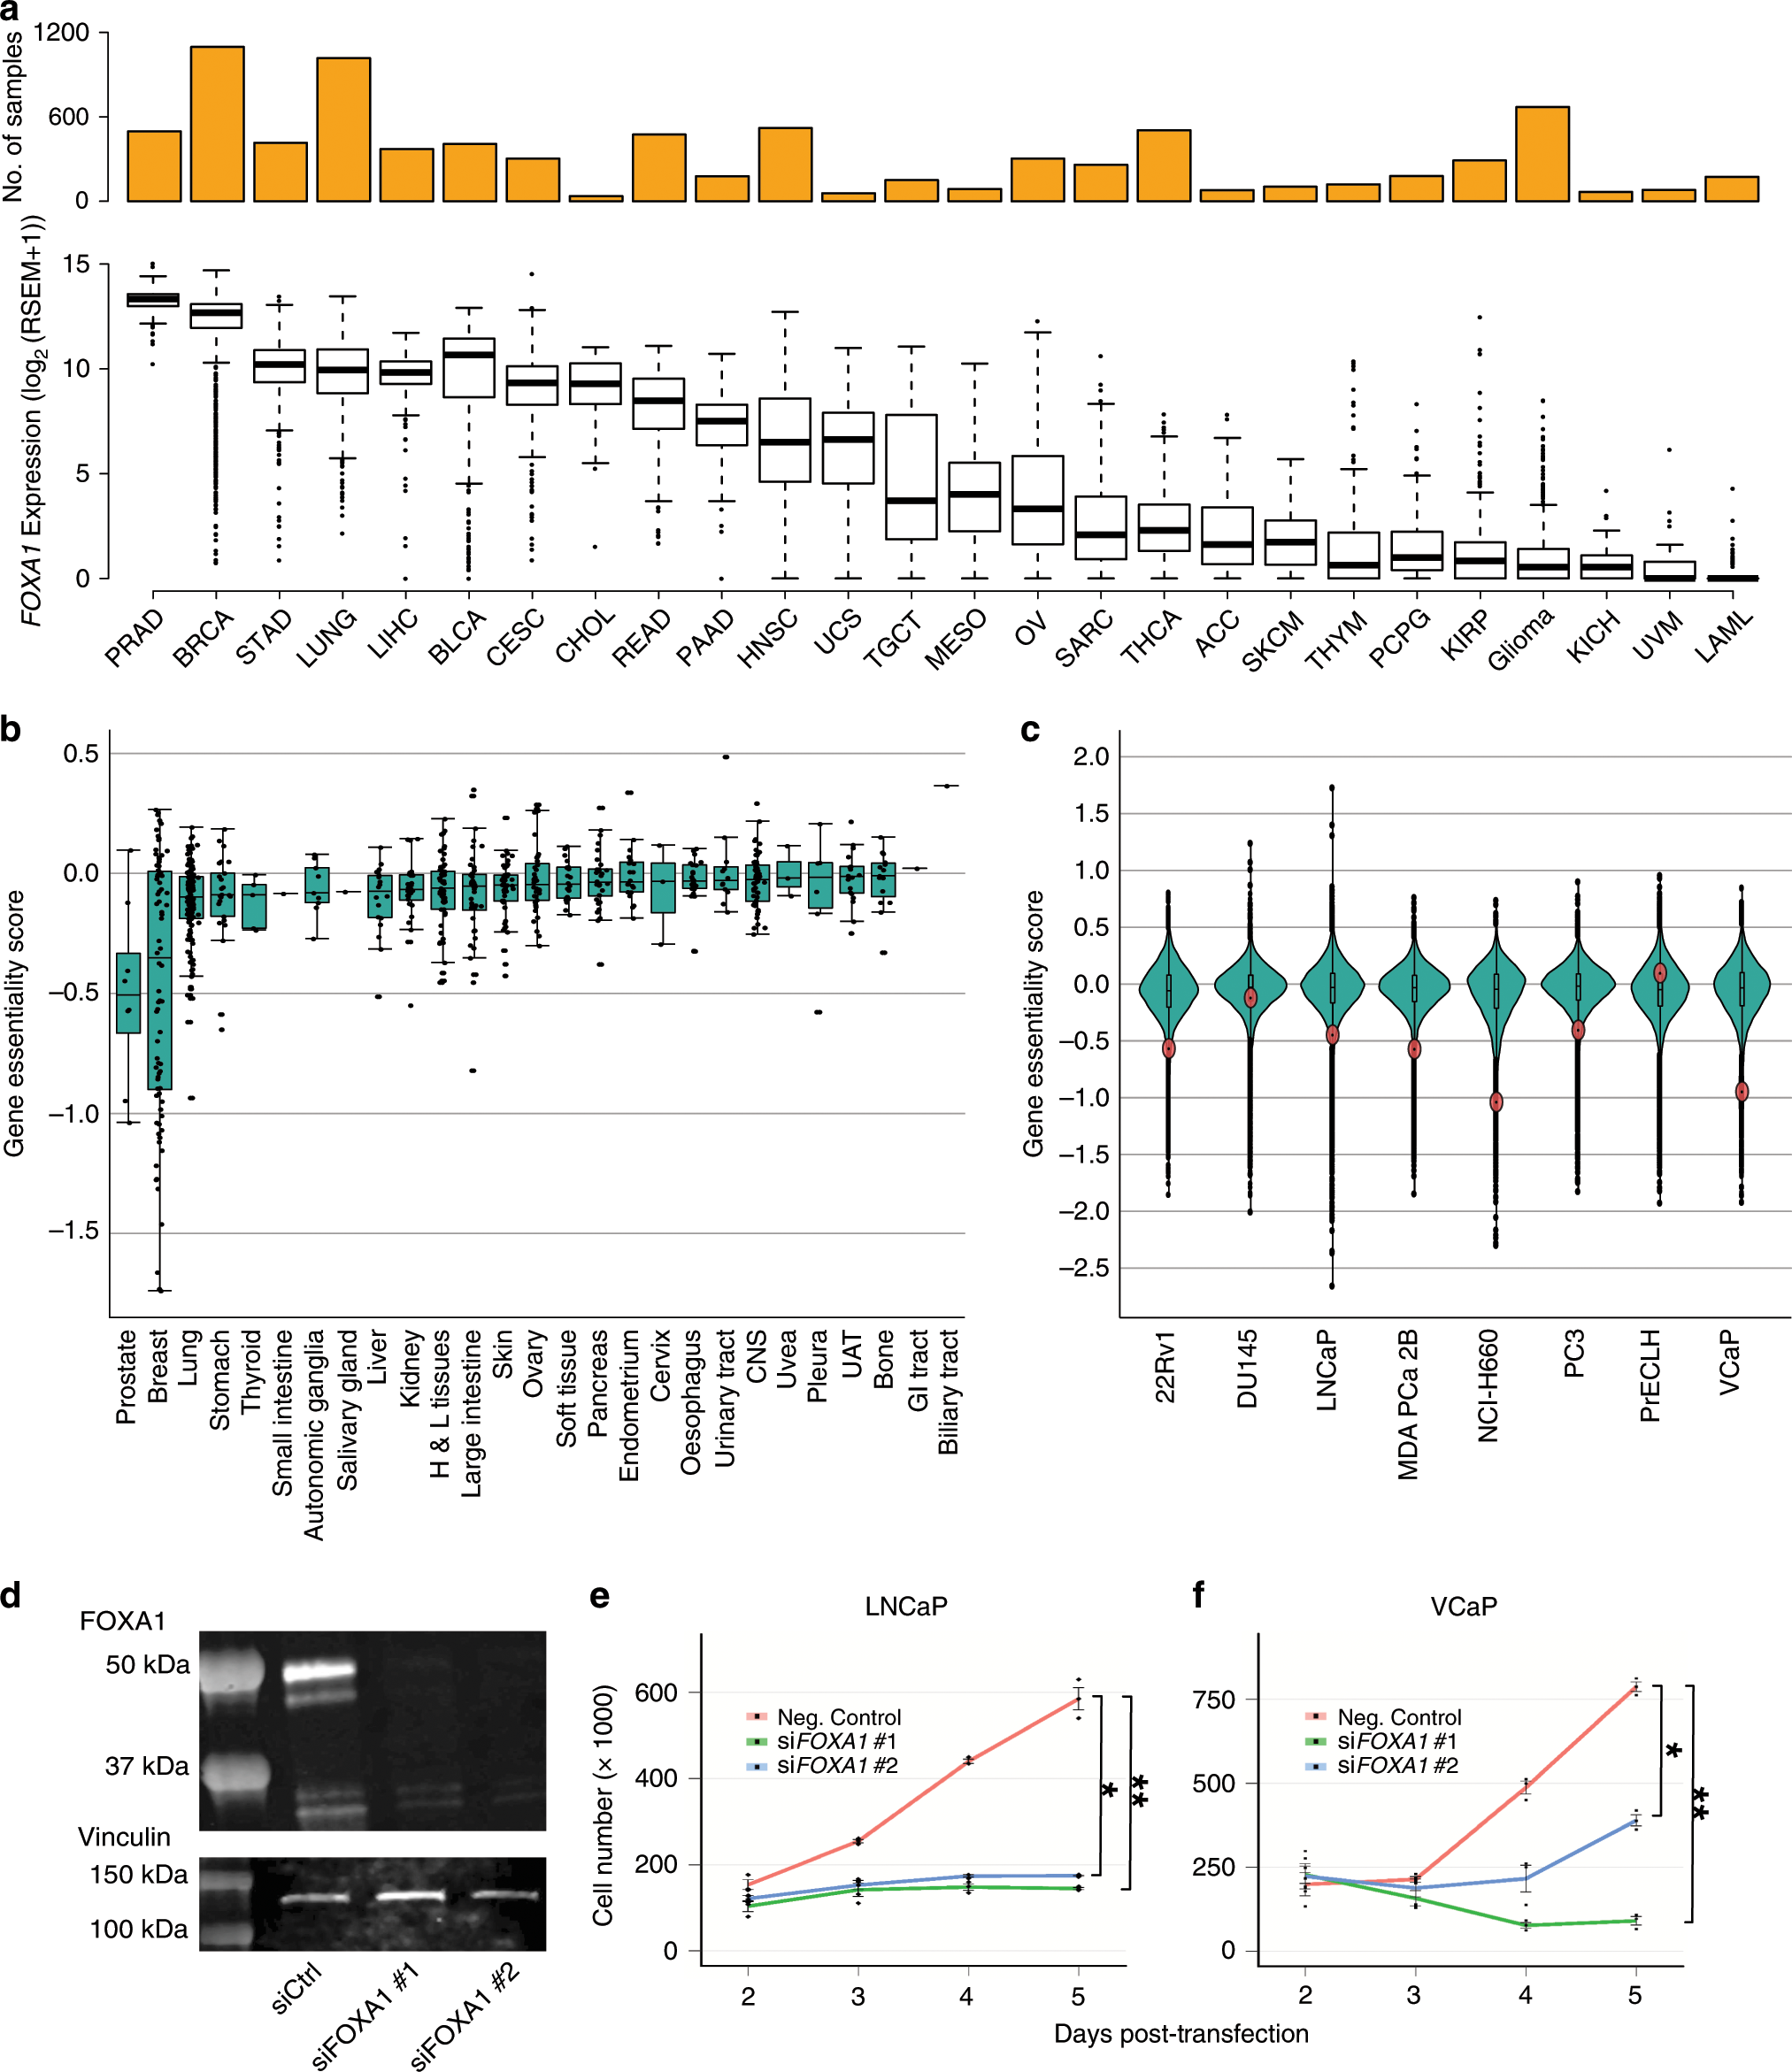
\includegraphics[width=0.95\textwidth]{Fig1.png}
  \caption{\textbf{FOXA1 is highly expressed in prostate cancer and essential for prostate cancer cell proliferation.} \textbf{a}. The mRNA expression of FOXA1 across tumour types ($n = 26$) from RNA-seq data of TCGA. \textbf{b}. FOXA1 essentiality mediated through RNAi across various cell lines ($n=707$) from DEPMAP. Gene essentiality scores are normalized Z-scores. Higher scores indicate less essential, and lower scores indicate more essential for cell proliferation. X-axis indicate tissue of origin for each cell line tested. Each dot indicates one cell line. \textbf{c}. Gene essentiality mediated through RNAi across prostate cancer cell lines ($n=8$) from DEPMAP. Each dot indicates one gene, red indicates FOXA1. \textbf{d}. Representative Western blot against FOXA1 in LNCaP cells 5 days post-transfection of non-targeting siRNA and two independent siRNA targeting FOXA1. \textbf{e}. Cell proliferation assay conducted in LNCaP cells upon siRNA-mediated knockdown of FOXA1 across 5 days. \textbf{f}. Cell proliferation assay conducted in VCaP cells upon siRNA-mediated knockdown of FOXA1 across 5 days. Error bars indicate $\pm$ s.d. $n=3$ independent experiments. Mann-Whitney U test, * $p < 0.05$, ** $p < 0.01$.}
  \label{fig:FOXA1_fig1}
\end{figure}

Following up on FOXA1 mRNA expression levels, we interrogated the essentiality of FOXA1 for prostate cancer cell growth.
RNAi-mediated essentiality screens compiled in DEPMAP show that FOXA1 lies in the 94th percentile across 6 of the 8 available prostate cancer cell lines: 22Rv1, LNCaP, MDA PCa 2B, NCI-H660, PC3, and VCaP cells (\Cref{fig:FOXA1_fig1}b-c).
The median RNAi-mediated essentiality score for all prostate cell lines is significantly lower than all other cell lines, suggesting that FOXA1 is especially essential for prostate cancer cell proliferation (permutation test, $p = 1 \cdot 10^{-6}$, see Methods) (\Cref{fig:FOXA1_figs3}a).
Growth assays in LNCaP and VCaP cells following FOXA1 knockdown using two independent siRNAs (\Cref{fig:FOXA1_fig1}d, \Cref{fig:FOXA1_figs3}b) show significant growth inhibition in LNCaP (siRNA \#1: 4-fold, siRNA \#2: 3.35-fold) and VCaP (siRNA \#1: 8.7-fold, siRNA \#2: 2-fold) cells five days post-transfection (Mann-Whitney U Test, $p<0.05$; \Cref{fig:FOXA1_fig1}e-f).
In accordance with previous reports, our results using essentiality datasets followed by knockdown validation reveals that FOXA1 is oncogenic and essential for prostate cancer cell proliferation.

% \subsection{Identifying putative \emph{FOXA1} CREs}

